\section{Auswertung}
\label{sec:Auswertung}
% Sämtliche im Folgenden durchgeführten Ausgleichsrechnungen werden mit der \emph{curve fit} Funktion aus dem für \emph{Python} geschriebenen package \emph{NumPy}\cite{scipy} durchgeführt. Fehlerrechnungen werden mit dem für \emph{Python} geschriebenen package \emph{Uncertainties}\cite{uncertainties} ausgeführt.

\subsection{Erzeugung von amplitudenmodulierten Schwingungen mit Hilfe eines
Ringmodulators}
In Abbildung \ref{fig:plot} ist das Signal einer amplitudenmodulierten
Schwingung dargestellt. Das Signal wird wie in Kapitel \ref{sec:Durchführung}
beschrieben erzeugt.

\begin{figure}
  \centering
  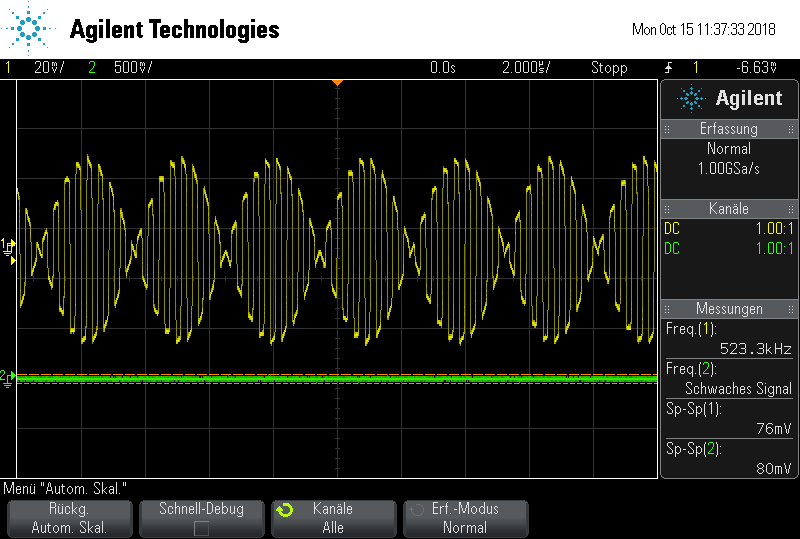
\includegraphics[width=0.7\linewidth]{ressources/scope_451.png}
  \caption{Darstellung des Modulationssignals des Ringmodulators.}
  \label{fig:plot}
\end{figure}
Für die Modulation werden zwei Sinusspannungen verschiedener Frequenzen und
Spannungen verwendet.
Für die Spannung des Trägersignals wurde eine Spannung von 40$\,$mV und eine
Frequenz von 2.87$\,$MHz
verwendet, die Modulationsspannung betrug 38$\,$mV mit einer Frequenz von
172.12$\,$kHz. Zusätzlich zu
dem modulierten Spannungsverlauf wurde das Frequenzspektrum des
Signal aufgenommen. Aus diesem Spektrum, vgl. Abbildung \ref{spek1}, lassen sich
die Frequenzen $\nu_\text{T},\nu_\text{L}=\nu_\text{T}-\nu_\text{M}$ und
$\nu_\text{R}=\nu_\text{T}+\nu_\text{M}$ bestimmen.
Die zentrale Frequenz $\nu_\text{z}=2.879\,$MHz, welches Peak 3 des
Frequenzspektrums entspricht, lässt sich als Trägerfrequenz interpretieren.
Die Frequenzen $\nu_\text{L}$ und $\nu_\text{R}$ entsprechen den Frequenzen
$\nu_\text{T}-\nu_\text{M}$ und $\nu_\text{T}+\nu_\text{R}$ und können den
Peak 1/2 im Frequenzspektrum zugeordnet werden. Was zusätzlich auffällt ist das
die Amplitude von $\nu_\text{z}$ deutlich abgeschwächt ist. Dieses lässt sich
auf die Trägerunterdrückung zurückführen.

\begin{figure}
  \centering
  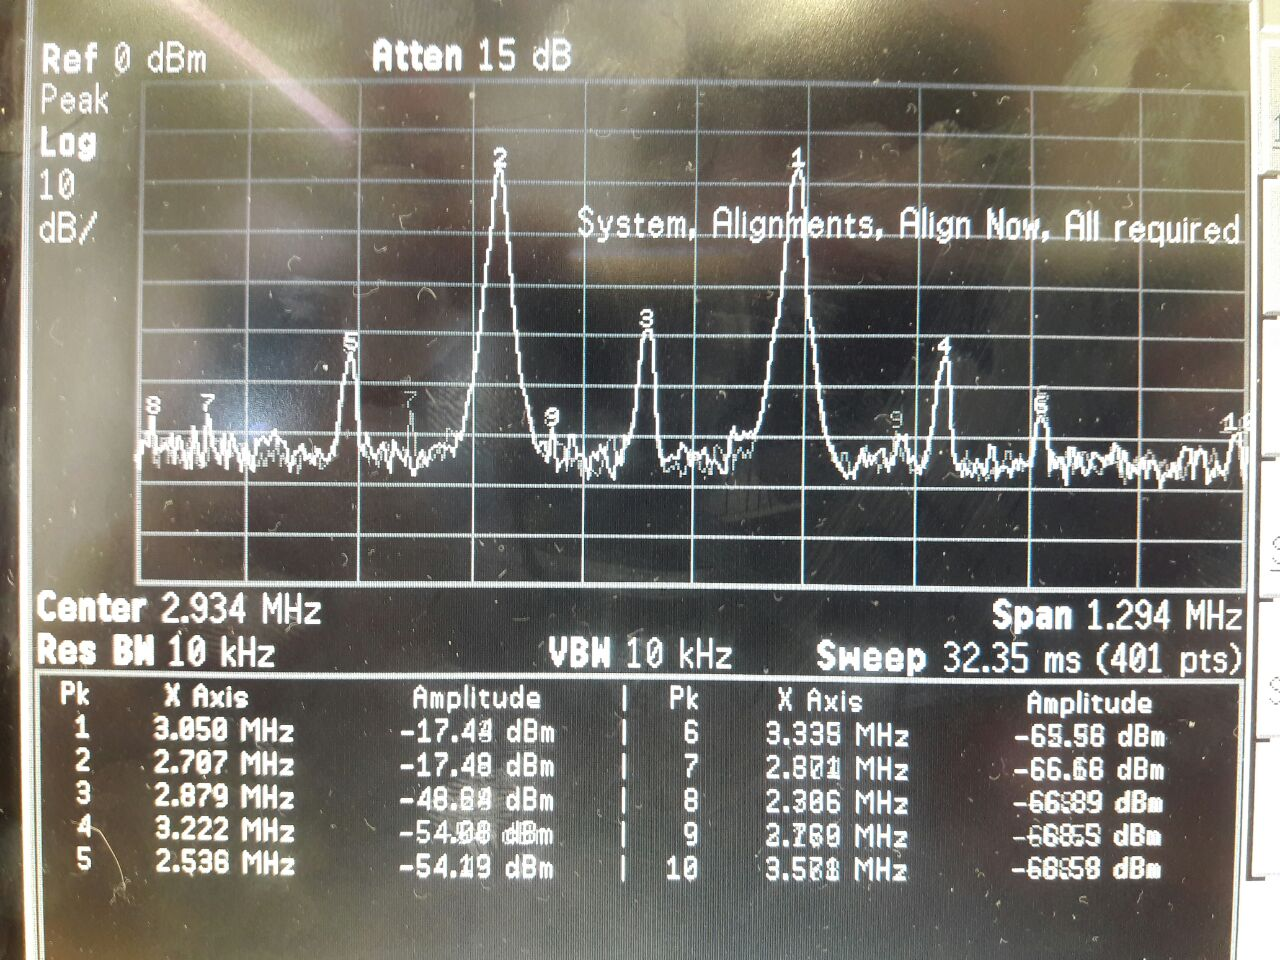
\includegraphics[width=0.7\linewidth]{ressources/photo5384285734183217712.jpg}
  \caption{Das Frequenzspektrum des amplituden modulierten Signals des Ringmodulators.}
  \label{spek1}
\end{figure}

\subsection{Erzeugung amplitudenmodulierter Schwingungen mit Hilfe einer Diode}
Zur Modulation eines ampltiduenmodulierten Signals mit Trägerabstrahlung wird eine
einfache Diode verwendet. Das so aufgenommene Signal ist in Abbildung
\ref{fig:plot2} zu sehen.
Ziel ist die Bestimmung des Modulationsgerades $m$, welcher durch die
maximal und minimal Werte des modulierten Signales bestimmt werden kann:
\begin{equation}
m=\frac{U_\text{max}-U_\text{min}}{U_\text{max}+U_\text{min}}.
\end{equation}
Die maximal und minimal Werte der Spannungen wurden mit Hilfe der Coursor
ausgelesen werden, sie werden unten rechts im aufgenommenen Bild \ref{fig:plot2}
angezeigt.
\begin{equation}
    U_\text{unten}=(45.750\pm 0.05)\,\text{mV} \quad \quad
    U_\text{max}=(83.750 \pm 0.05) \,\text{mV}
\end{equation}
Die angenommenen Unsicherheiten sind durch die endliche Ungenauigkeit des Oszilloskop gegeben.
Der resultierende Modulationsgrad liegt bei
\begin{equation}
    \label{mod1}
 m=0.2934 \pm 0.0006.
\end{equation}
\begin{figure}
  \centering
  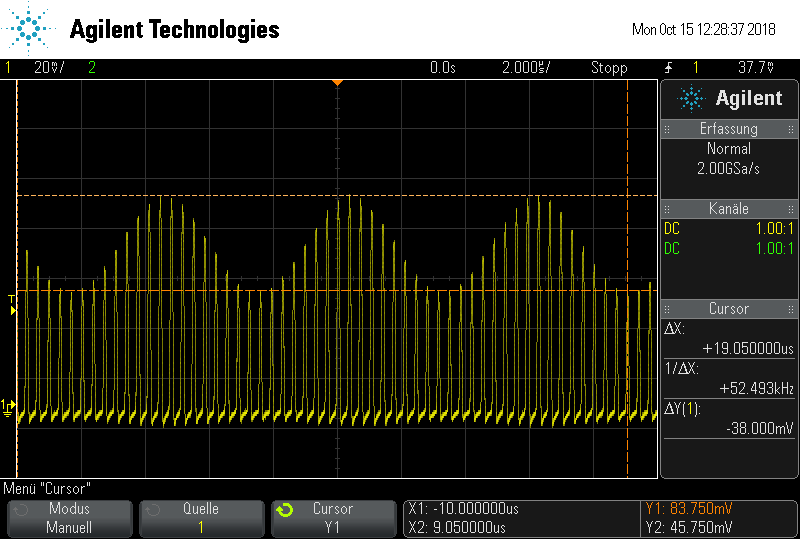
\includegraphics[width=0.7\linewidth]{ressources/scope_453.png}
  \caption{Darstellung des Modulationssignals der Diode.}
  \label{fig:plot2}
\end{figure}
Des Weiteren wurde das Signal des Frequenzspektrum aufgenommen, welches in
Abbildung \ref{spek2} zusehen ist. Die ersten 5 Maxima können deutlich als
solche identifiziert werden und sind in der Tabelle \ref{Tab1} aufgelistet.
Es werden die gemessenen Frequenzen mit den theoretisch bestimmten verglichen
und die Abweichung in $\%$  angegeben.
 \begin{table}
   \centering
   \caption{Die entnommenen Werte des Frequenzspektrums \ref{spek2}, zusätzlich
   die theoretisch berechneten Vorhersagen für die Oberwellen und deren
   Abweichungen zur Theorie.}
   \label{Tab1}
   \begin{tabular}{c|c|c|c}
     \toprule
$\text{Peak Nr.}$& $\nu_\text{gem}$ in Mhz & $\nu_\text{theo}$ in Mhz & Abweichug in \% \\
     \midrule
     1  & 2.879 &$\nu_\text{T}=$2.88 & 0.3\% \\
     2  & 3.050 &$\nu_\text{T}+\nu_\text{M}$= 3.051 & 0.03\% \\
     3  & 2.707  & $\nu_\text{T}-\nu_\text{M}=$2.708 & 0.03\%\\
     4  & 3.222 &$\nu_\text{T}+2\nu_\text{M}$= 3.224  & 0.06 \% \\
     5  & 2.536 & $\nu_\text{T}-2\nu_\text{M}$=2.536  & 0\%  \\
     \bottomrule
   \end{tabular}
 \end{table}
Der Modulationsgrad kann zusätzlich über die Leistung der aufgenommenen Frequenzen
bestimmt werden. Dafür muss zuerst die Amplitude in Leistung umgerechnet werden,
hierfür wurde die folgende Formel verwendet

\begin{align}
 P= 10\cdot ^{\frac{L}{10 \text{dBm}}}1\,\cdot  \text{mW}.
\label{watt}
\end{align}
Die Amplitude $L$ ist in Dezibel Milliwatt angegeben und die resulierende Leistung
ist folglich in Watt angegeben. Der Modulationsgrad kann über
die Beziehung $U^2= PR$ und einem konstanten Widerstand und bekannter
Leistung berechnet werden. Es ergibt sich eine Beziehung für den Modulationsgrad
$$m_{\pm} = 2 \sqrt{ \frac{ P_{\omega_\text{T}\pm \omega_\text{M}}}{P_{\omega_{\text{T}}}} }=
2\sqrt{ \frac{10 \frac{L_{\omega_\text{T}\pm \omega_\text{M}}}{10\,\text{dBm}}\,1\cdot \text{mW}}{ 10 \frac{L_{\omega_\text{T}}}{10\,\text{dBm}}\,1\cdot \text{mW}} }.$$
Mit den Amplituden aus den Frequenzspektrum.


\begin{align}
     \nonumber
    L_1=L_{\omega_{\text{T}}}=-19.85 \, \text{dBm}\\
    \nonumber
    L_2=L_{\omega_{\text{T}}-\omega_{\text{M}}}=-32.78 \, \text{dBm}\\
    \nonumber
    L_3=L_{\omega_{\text{T}}+\omega_{\text{M}}}=-32.86 \, \text{dBm}
\end{align}
ergeben sich folgende Werte für die Modulationsgerade:
$$m_{\omega_{\text{T}}-\omega_{\text{M}}}=0.45 \quad \quad m_{\omega_{\text{T}}+\omega_{\text{M}}}=0.44.$$

\begin{equation}
        \label{mod2}
        m=0.45 \pm 0.01
\end{equation}
\begin{figure}
  \centering
  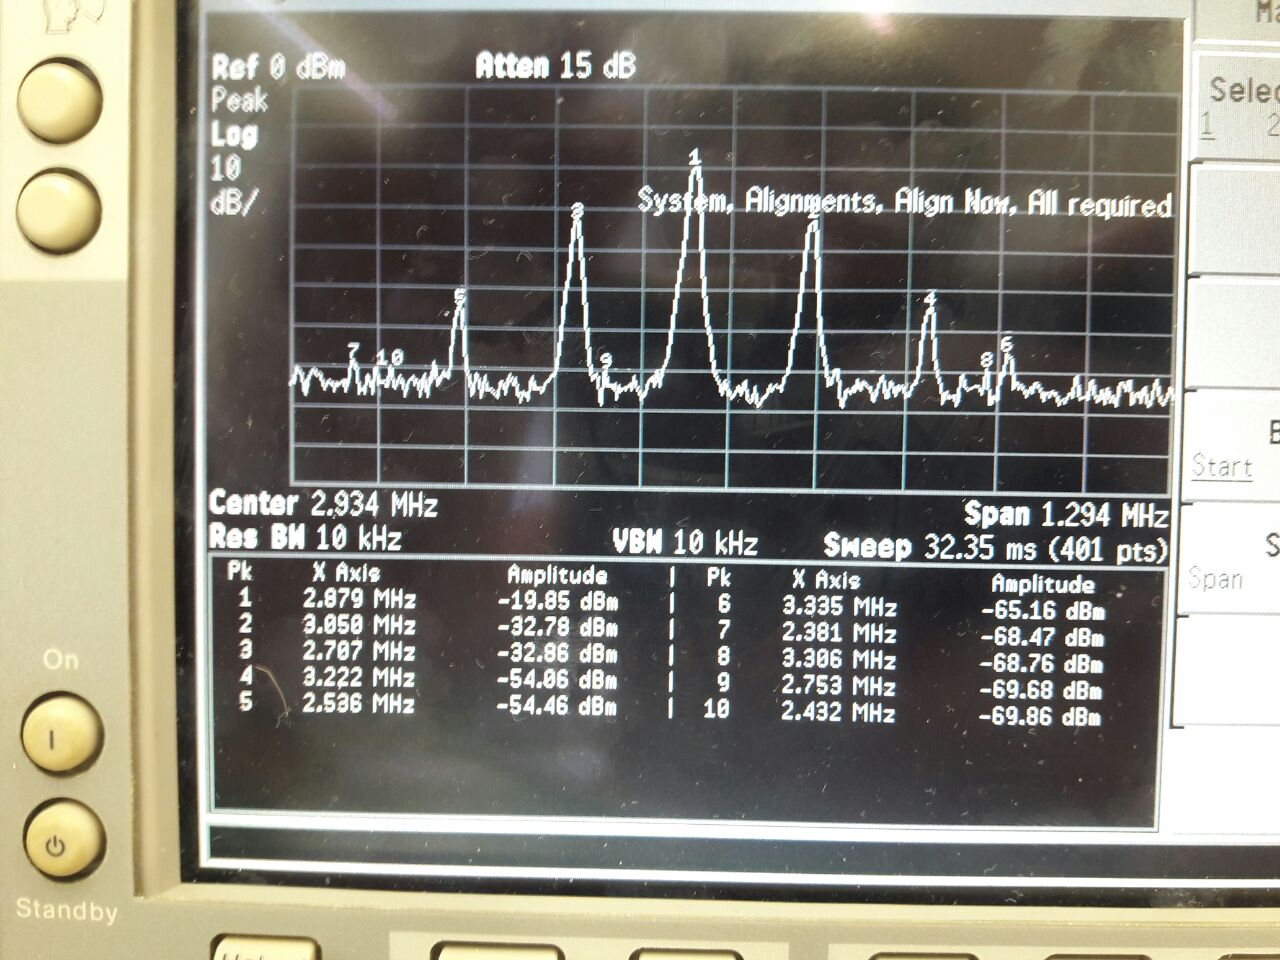
\includegraphics[width=0.7\linewidth]{ressources/photo5384285734183217711.jpg}
  \caption{Das Frequenzspektrum des amplituden modulierten Signals der Diode.}
  \label{spek2}
\end{figure}


\subsection{Erzeugung einer frequenzmodulierten Schwingung}
Zur Modulierung des Signals wird nun frequenzmodulierten Schwingungen betrachtet, das Trägersignal
hat eine Spannung von $U_\text{T}=(410.925\pm 0.025)\,\text{mV}$ und einer Frequenz von
$\nu_\text{T}=1.26 \, \text{MHz}$. Das Modulationssignal hat eine Spannung von
$U_\text{M}=350\,$mV und eine Frequenz von $\nu_\text{M}=125\,$kHz.
Das so modulierte Signal ist in Abbildung \ref{sig1} zu sehen, für die
weitere Aufgabenteile wird eine Detailaufnahme des zentralen Bereiche aus
Abbildung \ref{sig1} aufgenommen. Diese ist in Abbildung \ref{sig2} dargestellt,
hier ist die Verschmierung genauer zu sehen.\\

\begin{figure}
  \centering
  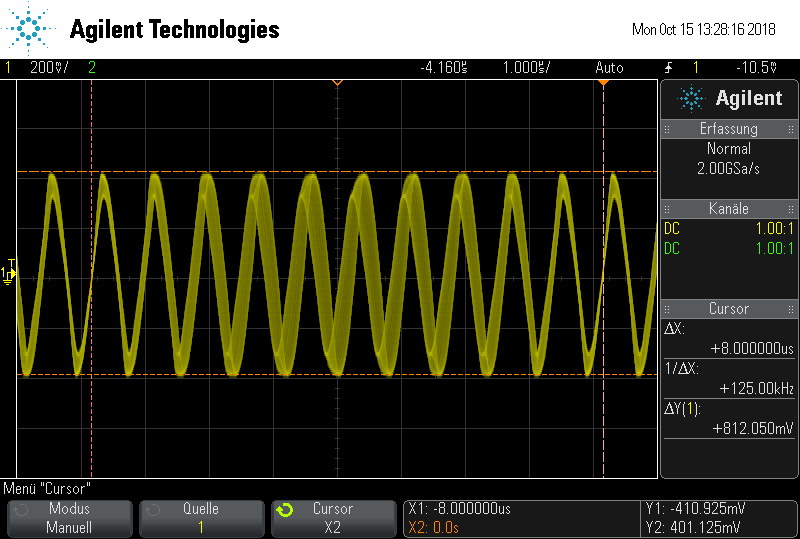
\includegraphics[width=0.7\linewidth]{ressources/scope_455.png}
  \caption{Darstellung des frequenzmodulierten Signals. Der Effekt der
  Verschmierung ist innerhalb der aufgenommenen Periode zu erkennen.}
  \label{sig1}
\end{figure}
\begin{figure}
  \centering
  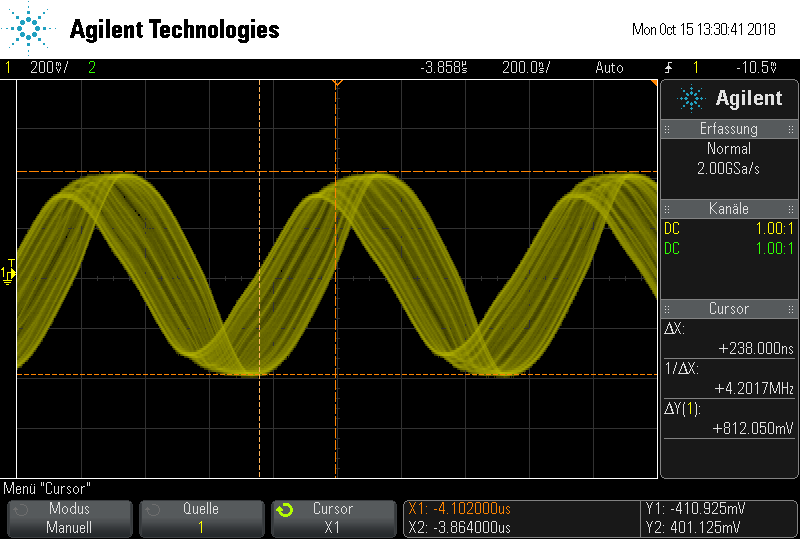
\includegraphics[width=0.7\linewidth]{ressources/scope_456.png}
  \caption{Detailaufname des frequenzmodulierten Signals, die
  Cursor kennzeichnen die Breite der Verschmierung.}
  \label{sig2}
\end{figure}
Ziel ist es, mit Hilfe der Verschmierung und der Frequenz des Trägersignals
einen Zusammmenhang zum Modulationsgrad herzuleiten. Dafür wird zuerst
die Verschmierung genauer Vermessen. Mit Hilfe der Cursor wurde die
Verschmierung zu
$$\Delta T = (238\pm 10)\, \text{ns}$$
genau bestimmt. Dabei ist $\pm 10\,$ns die angenommene Unsicherheit.

Für die Berechnung des Frequenzhubes und des Modulationsgrades darf die
Momentanfrequenz keine Zeitabhängigkeit mehr enthalten. Dazu wird bei der
Bestimmung der Momentanfrequenz über eine halbe Peridode gemittelt, dies
hat zur Folge das die Zeitabhängigkeit verschwindet. Damit folgt:
$$\bar{\nu}(\phi_0)=\frac{2}{T} \int_0^{T/2} \frac{\omega_\text{T}}{2\pi}
[1-m\cdot \sin (\omega_\text{M}t+ \phi_0)]=\frac{\omega_\text{T}}{2\pi}-
\frac{\omega_\text{T}\cdot m}{\pi^2}\cos(\phi_0)$$

Aufgrund des $\cos(\phi_0)$ gibt es einen Bereich, der die
gemittelte Frequenzen aus der Frequenzmodulation annehmen können. Es lässt
sich jedoch eine maximale und minimale Frequenz angeben:
\begin{align}
\bar{\nu_{\text{min}}}=\bar(\nu)(\phi_0=0)&=\frac{\omega T}{2\pi}-\frac{\omega \cdot m}{\pi^2}\\
\bar{\nu_{\text{max}}}=\bar(\nu)(\phi_0=\phi_0)&=\frac{\omega T}{2\pi}+\frac{\omega \cdot m}{\pi^2}
\end{align}
Der Modulationsgrad lässt sich nun über die Beziehung



\begin{align}
    \nonumber
\Delta T'=T_\text{max}-T_\text{min}=\frac{1}{\nu_\text{min}}-\frac{1}{\nu_\text{max}}\\
\nonumber
=\frac{1}{\frac{\omega T}{2\pi}-\frac{\omega \cdot m}{\pi^2}}-
\nonumber
 \frac{1}{\frac{\omega T}{2\pi}+\frac{\omega \cdot m}{\pi^2}}\\
 \nonumber
 \Leftrightarrow m^2+ \frac{2\pi^2}{\omega_\text{T} \Delta T'}m-\frac{\pi^2}{4}=0\\
 m_\pm=-\frac{\pi}{4\nu_\text{M}\Delta T}\pm\sqrt{\frac{\pi^2}{16\nu_\text{M}^2 \Delta T^2} +\frac{\pi^2}{4}}.
\end{align}
bestimmen. Dabei muss berücksichtig werden, dass nur positive Werte für den
Modulationsgrad sinnvoll sind. Des Weiteren ist $\Delta T'=2\nu_\text{M}/ \nu_\text{T}\Delta T$
die mittlere Verschmierung pro halb Schwingung. Setzt man nun die Werte ein, ergibt
sich für den Modulationsgrad
$$m= 0.606 \pm 0.002$$
Mit Hilfe des Modulationsgrades kann nun der Frequnezhub berechnet werden.
$$ \Delta \nu= m \nu_\text{T}= (76.4 \pm 0.2)\, \text{kHz}$$
Außerdem kann durch die Bestimmung des Modulationsgrad
gezeigt werden, dass die Schmalbandnäherung $$ m\frac{\omega_\text{T}}{\omega_\text{M}}\ll 1$$
nicht gut erfüllt ist.\\
Alternativ soll der Modulationsgrad über das Frequenzspekturm bestimmt werden.
Dazu werden die Amplituden der gemessenen Frequenzen
in die Leistung umgerechnet und über die Gleichung
$$ m= 2\frac{\nu_\text{M}}{\nu_\text{T}} \sqrt{\frac{P_{\omega_\text{T}} \pm \omega_\text{W}}{P_{\omega_\text{T}}} } $$
\begin{figure}
  \centering
  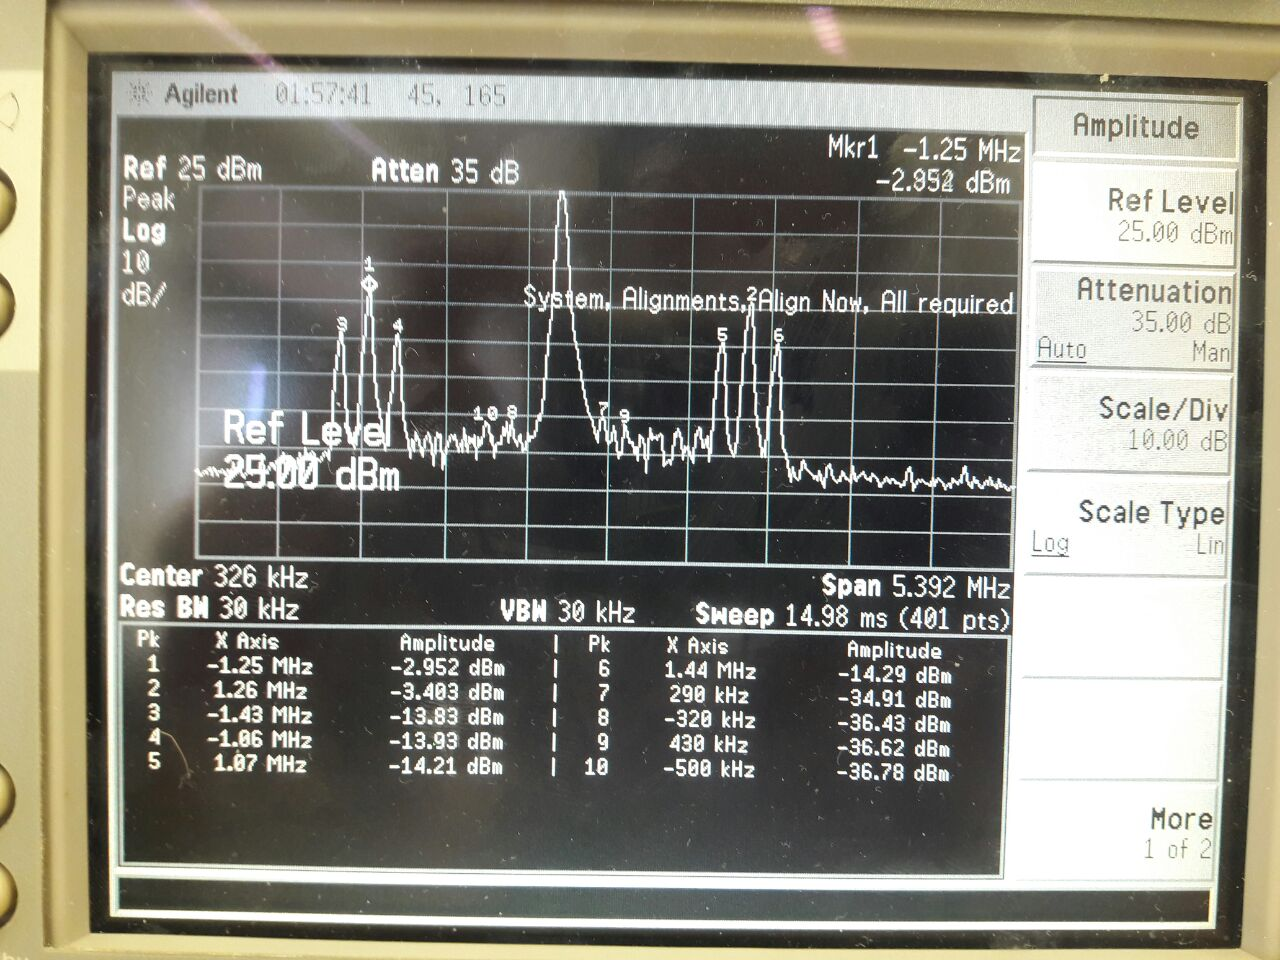
\includegraphics[width=0.7\linewidth]{ressources/photo5384285734183217710.jpg}
  \caption{Frequenzspektrum des frequenzmodulierten Signals.}
  \label{spek3}
\end{figure}
Die Amplituden der Frequenzen sind:
\begin{align}
    L_2=L_{\omega_{\text{T}}}=-3.403 \, \text{dBm}\\
    L_5=L_{\omega_{\text{T}}-\omega_{\text{M}}}=-14.21 \, \text{dBm}\\
    L_6=L_{\omega_{\text{T}}+\omega_{\text{M}}}=-14.29 \, \text{dBm}\\
\end{align}
diese werden mit Hilfe der Formel \ref{watt} in die entsprechenden mW Werte
umgerechnet.
Damit ergeben sich folgende Werte für die Modulationsgrade
$$ m_+= 0.576 \quad \quad \quad m_-=0.571$$
$$\rightarrow m= 0.574 \pm 0.003$$

\subsection{Phasenabhängigkeit der Ringmodulatorspannung}

Es soll gezeigt werden, dass die Gleichspannug des Ringmodulators eine
Abhängigkeit zur Phasendifferenz zur Eingangspannung aufweißt. Für diese
Messung wird die Eingangspannung $U_\text{E}$ und die Spannung nach dem
Tiefpass ($U_\text{TP})$ aufgenommen.
Um die Phasenabhängigkeit des Ringmodulators zu überprüfen, müssen zuerst
die aufgenommenen Frequenzen $f$ in die Phase umgerechnet werden. Hier wird die
Gleichung
$$ \phi=2  \pi f T, \quad \quad \quad T=290\,\text{ns} $$
verwendet. Die Zeit $T=290\,$ns ist eine Phasendifferenz die manuell eingebaut wird.
In folgenden wird eine Funktionsanpassung der Form

$$ U_\text{norm}(\phi)=U_0\cos(b\phi +\phi_\text{off})+U_\text{off}$$
verwendet. Die aufgenommenen Daten und die berechnete Phase $\phi$ sind in der
Tabelle \ref{Tab3} aufgelisteted und in der Grafik \ref{fit1} dargestellt.
\begin{table}
  \centering
  \caption{Die entnommenen Werte des Frequenzspektrums \ref{spek2}, zusätzlich
  die theoretisch berechneten Vorhersagen für die Oberwellen und deren
  Abweichungen zur Theorie.}
  \label{Tab3}
  \begin{tabular}{c|c|c|c}
    \toprule
Frequenz $f$ in MHz & Spannung $U_T$ &Eingangspannung $U_\text{E}$& Phasenverschiebung $\Phi$\\
    \midrule
    1 & -0.002 & 1.35  & 1.82  \\
    1.2& 0.055 &1.27  & 2.19  \\
    1.4& 0.108 & 1.21 &  2.55 \\
    1.6& 0.163 & 1.27  & 2.92  \\
    1.8& 0.212 &1.11  & 3.28  \\
    2.0& 0.247  &1.08  & 3.64  \\
    2.2& 0.222 & 1.27  & 4.01  \\
    2.4&  0.176&  1.31  & 4.37  \\
    2.6&  0.127&  1.23  & 4.73  \\
    2.8& 0.07 & 1.37   &  5.10 \\
    3.0 &0.015 &1.38   &  5.47 \\
    3.2 &-0.04 &1.31  & 5.83  \\
    3.4 & -0.091& 1.33  & 6.20  \\
    3.6 &-0.145 &1.37   & 6.56  \\
    3.8 &-0.201 &1.19  & 6.92  \\
    4.0 &-0.244 &1.23  &  7.29 \\
    4.2 &-0.239 &1.41  & 7.65  \\
    4.4& -0.192 &1.35  & 8.02  \\
    4.6& -0.147 & 1.51  & 8.38   \\
    4.8& -0.094 &1.63  & 8.75  \\
    5.0& -0.029 &1.63 & 9.11  \\
    5.2& 0.019 &1.45 & 9.48  \\
    5.4& 0.068 &1.71 &  9.83 \\

    \bottomrule
  \end{tabular}
\end{table}


\begin{figure}
  \centering
  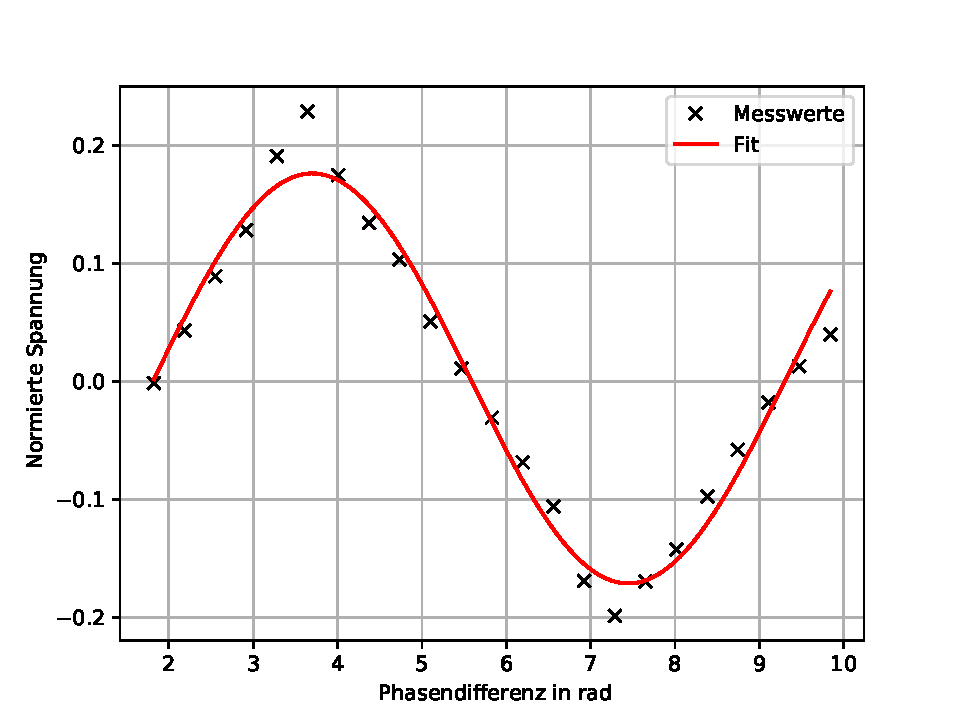
\includegraphics[width=0.7\linewidth]{build/plot.pdf}
  \caption{Darstellung der normierten Spannung $U$ und der Phase $\phi$ mit
  Ausgleichsfunktion.
  .}
  \label{fit1}
\end{figure}
Für die Parameter der Funktionsanpassung ergeben sich die Werte:
\begin{align}
U_0=&0.174 \pm 0.006\\
b=&0.84 \pm 0.01 \\
\phi_\text{off}=&3.18 \pm 0.09 \\
U_\text{off}=&0.003 \pm 0.004
\end{align}


\subsection{Demodulation einer amplitudenmodulierten Schwingung mit Hilfe eines
Ringmodulators}
Das Ziel ist hier die Demodulation des Signal mit Hilfe eines Ringmodulators.
Das demodulierte Signal ist in Abbildung \ref{gege} zu sehen. Es lässt
sich feststellen, dass bis auf eine Phasenverschienung und einer verringerten
Amplitude, sich das Signal, welches zuvor moduliert worden ist, demodulieren ließ. Die Spannung
des Modulationssignal liegt bei $U_\text{M}=119.5 \,\text{mV}$ und das demodulierte
Signal bei $U_\text{De}95.7\,\text{mV}$.

\begin{figure}
  \centering
  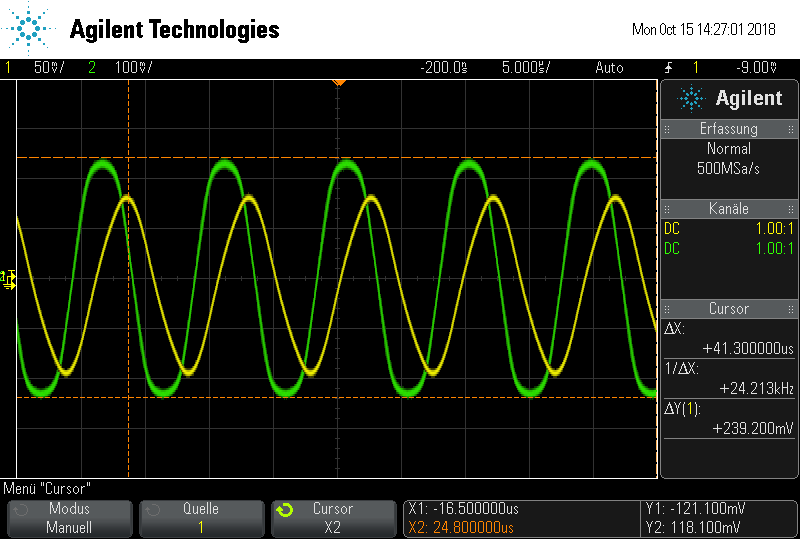
\includegraphics[width=0.7\linewidth]{ressources/scope_459.png}
  \caption{Darstellung des demodulierten Signal des Ringmodulators.}
  \label{gege}
\end{figure}

\subsection{Demodulation mit amplitudenmodulierten Spannung mit einer
Gleichrichterdiode}
Das amplitudenmodulierte Signal wird nach den einzelnen Bauteilen betrachtet.
Die Bilder \ref{vortp} und \ref{ntp} stellt das Signal vor und nach dem Tiefpass dar.
Die Frequenz des Trägersignals beträgt $\nu_\text{T}=1.90\,$MHz und das Modulatiosnsignal
besitzt eine Frequenz von $\nu_\text{M}=104.8\,$kHz.
Durch Betrachtung des demodulierten Signals wird deutlich, dass sich die
Amplitude deutlich verringert.Zu Beginn hat sie einen Wert von $U_\text{B}=470\,$mV
und fällt nach dem Tiefpass auf ca $U_\text{TP}=3.7\,$mV ab. Die Frequenz hat
sich jedoch von $\nu_\text{M}=104.8\,$kHz auf $\nu_\text{M}=209.6\,$kHz so gut wie
verdoppelt.
\begin{figure}
  \centering
  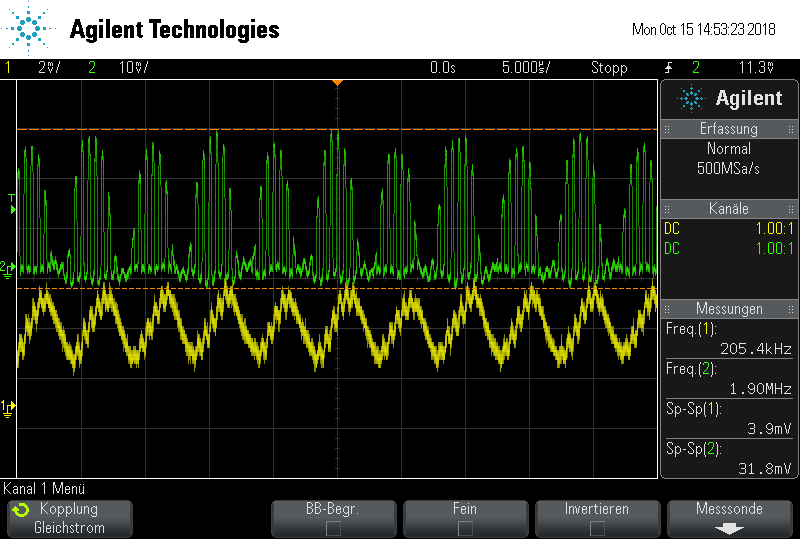
\includegraphics[width=0.7\linewidth]{ressources/scope_461.png}
  \caption{Ursprüngliches Modulationssignal und das Signal nach der Gleichrichterdiode.}
  \label{vortp}
\end{figure}

\begin{figure}
  \centering
  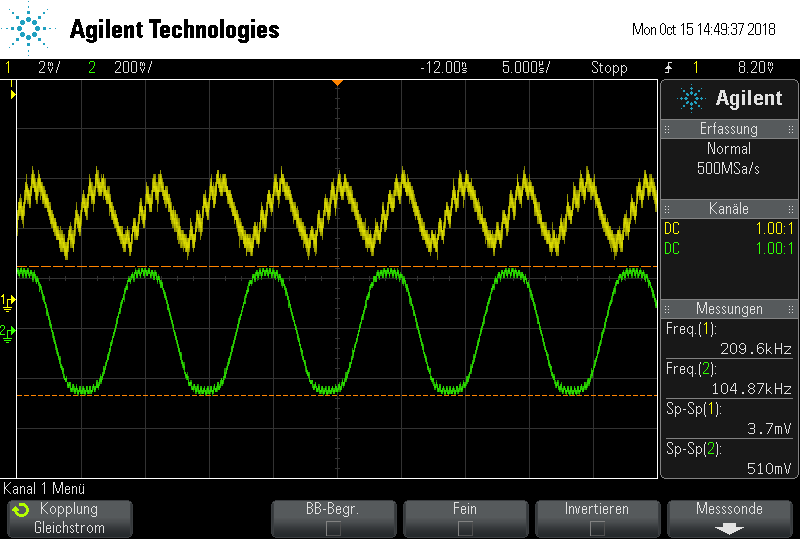
\includegraphics[width=0.7\linewidth]{ressources/scope_460.png}
  \caption{Darstellung des ursprünglichen Modulationssignals und das demodulierte Signal nach dem Tiefpass.}
  \label{ntp}
\end{figure}
\subsection{Demodulation einer frequenzmodulierten Schwingung}
Zur Untersuchung der Demodulation einer frequenzmodulierten Spannung werden
Aufnahmen der Spannungsverläufe nach jedem der verwendeten Bauteile angefertigt.
Bei dem ersten Schritt wird das frequenzmodulierte Signal in ein
amplitudenmoduliertes überführt, vgl. Abbildung \ref{fmd}. Anschließend
werden die unteren Halbwellen des Signal abgeschnitten, welches in Abbildung
\ref{halb} zusehen ist. Als letztes wird wieder ein Tiefpass verwendet.
Das Signal nach dem Tiefpass ist in der Grafik \ref{ntp2} dargestellt.
Die Frequenz des Signal ist bis auf eine vernachlässigebare Schwankung
von  $\nu_\text{M}=44.53\,$kHz auf $\nu_\text{M}=44.52\,$kHz gesunken und
das Signal wurde erfolgreich demoduliert. Die Amplitude
hingegen weist einen deutlichen Verlust der Spannung von $U=550\,$mV auf 5$\,$mV auf.


\begin{figure}
  \centering
  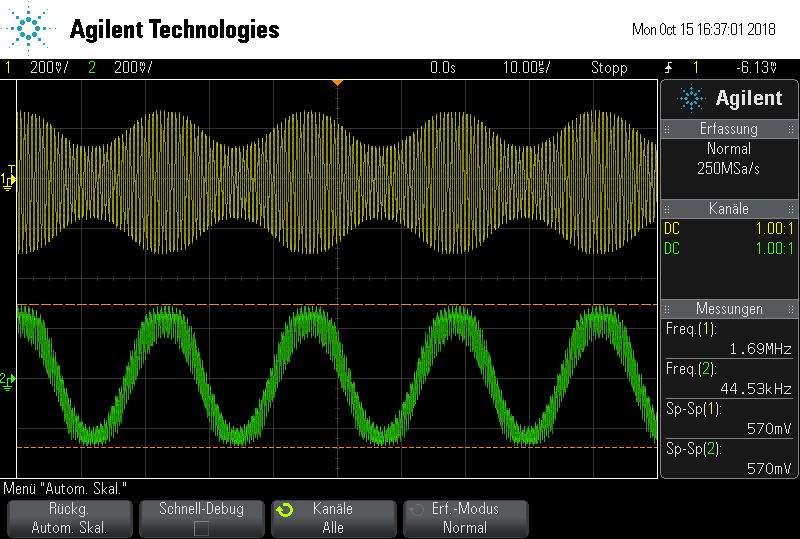
\includegraphics[width=0.7\linewidth]{ressources/scope_468.png}
  \caption{Darstellung des zu modulierende Signals vor und nach dem Schwingkreis.}
  \label{fmd}
\end{figure}
\begin{figure}
  \centering
  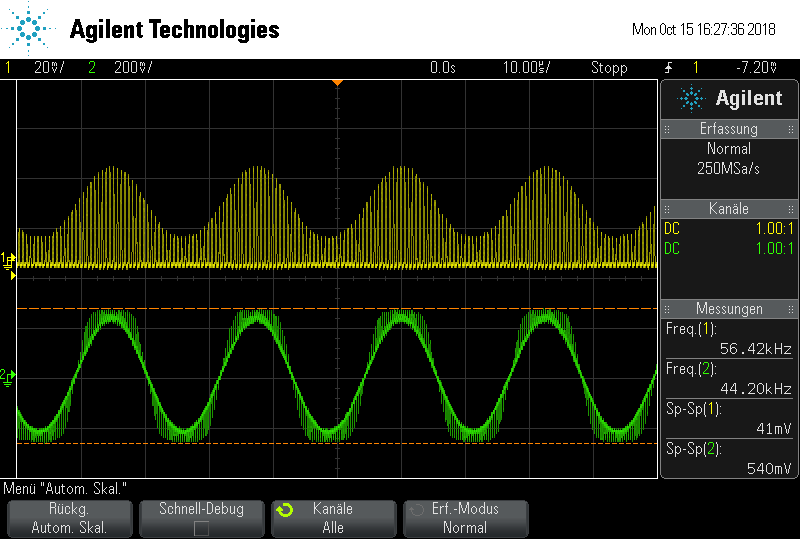
\includegraphics[width=0.7\linewidth]{ressources/scope_464.png}
  \caption{Signal nach abschneiden der unteren Halbwellen mit Hilfe einer Gleichrichterdiode.}
  \label{halb}
\end{figure}
\begin{figure}
  \centering
  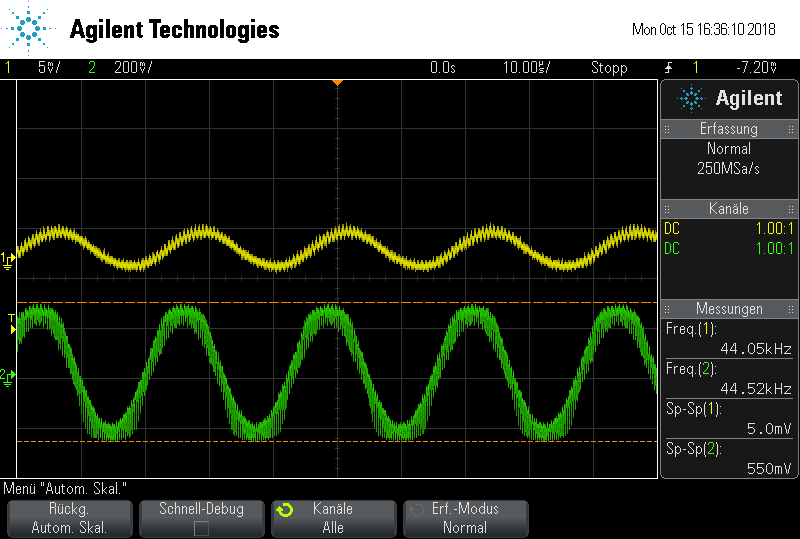
\includegraphics[width=0.7\linewidth]{ressources/scope_467.png}
  \caption{Darstellung des ursprünglichen Modulationssignals und das demodulierte Signal nach dem Tiefpass.}
  \label{ntp2}
\end{figure}


% % Exampl  es
% \begin{equation}
%   U(t) = a \sin(b t + c) + d
% \end{equation}
%
% \begin{align}
%   a &= \input{build/a.tex} \\
%   b &= \input{build/b.tex} \\
%   c &= \input{build/c.tex} \\
%   d &= \input{build/d.tex} .
% \end{align}
% Die Messdaten und das Ergebnis des Fits sind in Abbildung~\ref{fig:plot} geplottet.
%
% %Tabelle mit Messdaten
% \begin{table}
%   \centering
%   \caption{Messdaten.}
%   \label{tab:data}
%   \sisetup{parse-numbers=false}
%   \begin{tabular}{
% % format 1.3 bedeutet eine Stelle vorm Komma, 3 danach
%     S[table-format=1.3]
%     S[table-format=-1.2]
%     @{${}\pm{}$}
%     S[table-format=1.2]
%     @{\hspace*{3em}\hspace*{\tabcolsep}}
%     S[table-format=1.3]
%     S[table-format=-1.2]
%     @{${}\pm{}$}
%     S[table-format=1.2]
%   }
%     \toprule
%     {$t \:/\: \si{\milli\second}$} & \multicolumn{2}{c}{$U \:/\: \si{\kilo\volt}$\hspace*{3em}} &
%     {$t \:/\: \si{\milli\second}$} & \multicolumn{2}{c}{$U \:/\: \si{\kilo\volt}$} \\
%     \midrule
%     \input{build/table.tex}
%     \bottomrule
%   \end{tabular}
% \end{table}
%
% % Standard Plot
% \begin{figure}
%   \centering
%   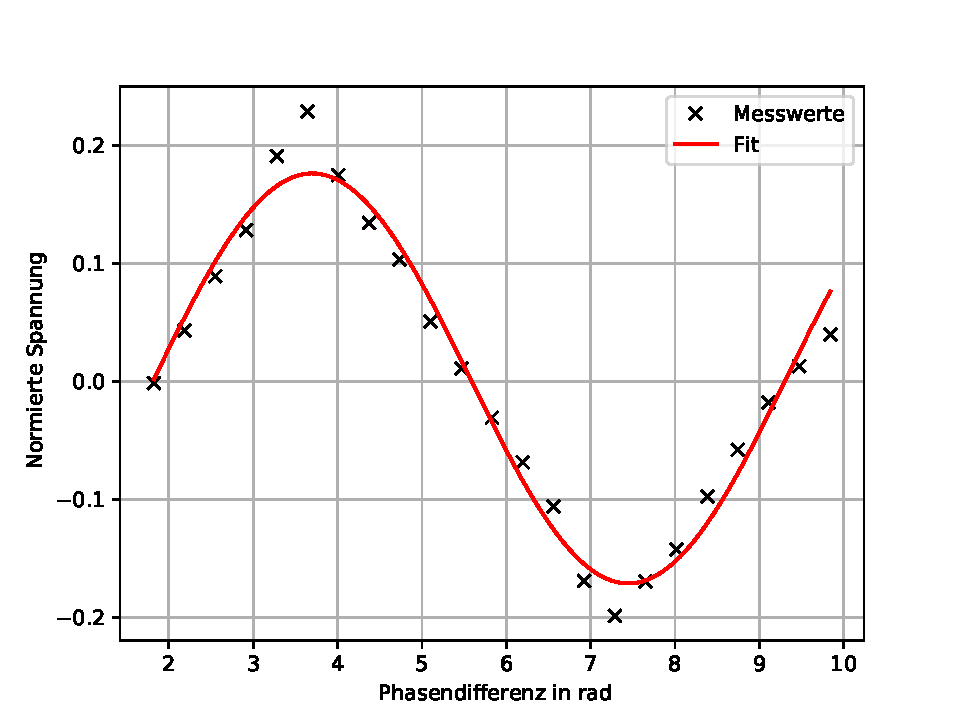
\includegraphics{build/plot.pdf}
%   \caption{Messdaten und Fitergebnis.}
%   \label{fig:plot}
% \end{figure}
%
% 2x2 Plot
% \begin{figure*}
%     \centering
%     \begin{subfigure}[b]{0.475\textwidth}
%         \centering
%         \includegraphics[width=\textwidth]{Abbildungen/Schaltung1.pdf}
%         \caption[]%
%         {{\small Schaltung 1.}}
%         \label{fig:Schaltung1}
%     \end{subfigure}
%     \hfill
%     \begin{subfigure}[b]{0.475\textwidth}
%         \centering
%         \includegraphics[width=\textwidth]{Abbildungen/Schaltung2.pdf}
%         \caption[]%
%         {{\small Schaltung 2.}}
%         \label{fig:Schaltung2}
%     \end{subfigure}
%     \vskip\baselineskip
%     \begin{subfigure}[b]{0.475\textwidth}
%         \centering
%         \includegraphics[width=\textwidth]{Abbildungen/Schaltung4.pdf}    % Zahlen vertauscht ... -.-
%         \caption[]%
%         {{\small Schaltung 3.}}
%         \label{fig:Schaltung3}
%     \end{subfigure}
%     \quad
%     \begin{subfigure}[b]{0.475\textwidth}
%         \centering
%         \includegraphics[width=\textwidth]{Abbildungen/Schaltung3.pdf}
%         \caption[]%
%         {{\small Schaltung 4.}}
%         \label{fig:Schaltung4}
%     \end{subfigure}
%     \caption[]
%     {Ersatzschaltbilder der verschiedenen Teilaufgaben.}
%     \label{fig:Schaltungen}
% \end{figure*}
